\documentclass[conference,a4paper]{IEEEtran}
\IEEEoverridecommandlockouts
\def\BibTeX{{\rm B\kern-.05em{\sc i\kern-.025em b}\kern-.08em
    T\kern-.1667em\lower.7ex\hbox{E}\kern-.125emX}}

% Language setting
% Replace `english' with e.g. `spanish' to change the document language
\usepackage[english]{babel}

% Set page size and margins
% Replace `letterpaper' with `a4paper' for UK/EU standard size
%\usepackage[letterpaper,top=2cm,bottom=2cm,left=3cm,right=3cm,marginparwidth=1.75cm]{geometry}

% Useful packages
\usepackage{amsmath}
\usepackage{graphicx}
\usepackage[colorlinks=true, allcolors=blue]{hyperref}

\title{Progress Report}
\author{Samuel~J.~Frost}

\begin{document}
\maketitle

\begin{abstract}
\textbf{Abstract.} Certainly! Here's a suggestion for how to being your PhD progress report. 
\end{abstract}

\section{Introduction}
simple as

\begin{figure}[htbp]
      \centering
      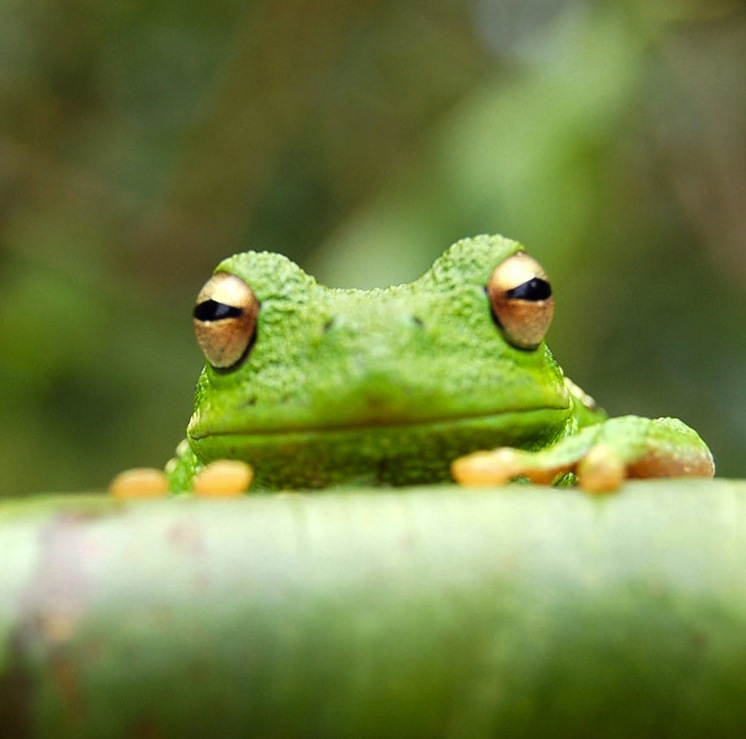
\includegraphics[width=0.25\linewidth]{frog.jpg}
      \caption{\label{fig:frog}wow he's literally me remember equations are part of sentences; don't forget}
      \end{figure}

\section{Some examples to get started}
Hmmmm testing


\subsection{How to create Sections and Subsections}

%\bibliographystyle{alpha}
%\bibliography{sample}

\end{document}